\documentclass[a4paper, 12pt, twoside]{report}
\usepackage[a4paper,left=25.4mm, right=25.4mm, top=25.4mm, bottom=25.4mm]{geometry}
\usepackage[utf8]{inputenc}
\usepackage{graphicx}

\renewcommand{\contentsname}{Cuprins}
\renewcommand{\listfigurename}{Figuri}

%list/enum
\usepackage{outlines}

%code
\usepackage{listings}
\usepackage{color}
\usepackage{inconsolata}
 
\definecolor{codegreen}{rgb}{0,0.6,0}
\definecolor{codegray}{rgb}{0.5,0.5,0.5}
\definecolor{codepurple}{rgb}{0.58,0,0.82}
\definecolor{backcolour}{rgb}{0.95,0.95,0.92}
\definecolor{comments}{rgb}{0,0.3,0}
 
\lstset{language=Go,
    backgroundcolor=\color{backcolour},  
    basicstyle=\ttfamily\footnotesize,
    keywordstyle=\color{blue}\ttfamily,
    stringstyle=\color{red}\ttfamily,
    commentstyle=\color{comments}\ttfamily,
    breakatwhitespace=false,         
    breaklines=true,                 
    captionpos=b,                    
    keepspaces=true,                 
    numbers=left,                    
    numbersep=5pt,                  
    showspaces=false,                
    showstringspaces=false,
    showtabs=false,                  
    tabsize=2
}
 

%titlesec and titleformat for chapters without 'chapter 1' tags
\usepackage{titlesec} 
\titleformat{\chapter}[display]
  {\normalfont\bfseries}{}{0pt}{\Huge}

%for clickable table of contents
\usepackage{hyperref}
\hypersetup{
    colorlinks,
    citecolor=black,
    filecolor=black,
    linkcolor=black,
    urlcolor=black
}

%for glossary of terms
\usepackage[acronym]{glossaries}
\makeglossaries
\newacronym{cups}{CUPS}{Common Unix Printing System}

\graphicspath{ {img/} }
\title{
	{Sistem de colectare și analiză a datelor din procesul de tipărire}\\
	{\large Universitatea Politehnica Timișoara}\\
	{
\includegraphics[width=50mm]{upt_logo.png}}
}
\author{Andrei Buruntia \\ andreiburuntia@gmail.com\\[1cm]{ Advisor: conf. dr. ing. Dan Cosma}}
\date{20-05-2018}
\begin{document}

\maketitle

\newpage\null\thispagestyle{empty}\newpage

\chapter*{Abstract}
În zilele noastre există o multitudine de imprimante și soluții de printing disponibile, fiecare cu interfața și setul ei de funcționalități. Această teză urmărește construirea unei platforme universale care să permită ascunderea imprimantelor după un strat de abstractizare suplimentar, oferind o singură interfață și posibilitatea de a furniza unei companii de printing date relevante sub formă de grafice.

Adresarea problemei anterior menționată necesită depășirea anumitor obstacole, trei dintre care fiind: abstractizarea imprimantei și a funcțiilor ei, integrarea imprimantelor moderne de orice fel, realizarea unor rapoarte închegate și coerente cu date extrase din procesul de printare, care să prezinte relevanță pentru utilizator, ideal permițând utilizatorului sa își creeze propria interfață, dupa nevoile și preferințele lui.

În consecință, lucrarea mea propune o soluție bazată pe \acrshort{cups}, care se ocupă de comunicațiile și controlul imprimantelor și de expunerea lor pe rețea. Acest lucru permite acoperirea unei game largi de imprimante, pastrearea complexității la un nivel relativ redus și accesarea informațiilor lower-level.

S-a considerat prioritară creerea unei platforme cap-coadă care sa nu restricționeze in vreun fel workflow-ul normal al unui utilizator.

Lucrarea arată potențialul folosirii tehnologiilor și sistemelor open-source la rezolvarea problemelor din ecosistemul corporate prin modificări si îmbunatațiri aduse acestora.

\newpage\null\thispagestyle{empty}\newpage

\chapter*{Declarație pe propria răspundere}
Subsemnatul Buruntia Andrei-Cristian, legitimat cu CI seria TZ nr. 080265, CNP 1950819165656, autorul lucrarii "Sistem de colectare și analiză a datelor din procesul de tipărire", elaborată în vederea susținerii examenului de finalizare a studiilor de licență organizat de către Facultatea de Automatică și Calculatoare din cadrul Universităţii Politehnica Timişoara, sesiunea iunie a anului universitar 2018, luând în considerare conţinutul art. 39 din RODPI – UPT, declar pe proprie răspundere, că această lucrare este rezultatul propriei activităţi intelectuale, nu conţine porţiuni plagiate, iar sursele bibliografice au fost folosite cu respectarea legislaţiei române şi a convenţiilor internaţionale privind drepturile de autor.

\bigskip

\noindent\begin{tabular}{ll}
\makebox[2.5in]{\hrulefill} & \makebox[2.5in]{\hrulefill}\\
Semnătură & Dată\\[8ex]% adds space between the two sets of signatures
\end{tabular}

\newpage\null\thispagestyle{empty}\newpage

\tableofcontents

\newpage\null\thispagestyle{empty}\newpage

\chapter{Introducere}

	\section{Context și motivație}
Océ, compania în care lucrez, activează în domeniul de printing, fiind subsidiar Canon. I companie se pune problema analizei și colectării datelor din procesul de imprimare. La propunerea companiei, am încercat sa abordez aceasta problema. Mai jos este prezentata mai pe larg problema, iar lucrarea urmărește propunerea unei idei de implementare a unu sistem care sa o rezolve. I aceasta documentație se va încerca detalierea asupra anumitor aspecte ale lucrării: dificultățile întâlnite, probleme de comunicare, constraint-uri de orice fel, etc.

	\section[Problema]{Problema \\ {\large Analiza și colectare de statistici despre procesul de imprimare}}

Pentru a putea optimiza costurile și procedeele de tipărire în cazul imprimantelor de format mare se dorește analiza și colectarea de statistici referitoare la: 
\begin{enumerate}
\item Cantitatea de cerneala folosita
\item Tipul de material pe care se face tiparire
\item Informatii despre tipul de culoare
\item Informatii despre metoda de finisare (capsare, copertare, lacuire. etc)
\end{enumerate}
Aceste informații trebuiesc agregate și afișate sub forma unor grafice care pot fi folosite de către utilizatori cat și de către compania Océ. Utilizatorii vor avea informații legate de costuri și timpi de execuție. Compania Océ poate folosi aceste informații în mod anonimizat pentru a culege informații legate de calitatea tipăririi și a a procesului cat și pentru an analiza în mod proactiv procesul de tipărire și a colecta informații despre modul în care imprimantele se comporta în timp și a preîntâmpina anumite defecțiuni.
Deoarece baza de imprimante este relative mare și nu toate imprimantele oferă în mod nativ informații despre consumabilele și cantitatea de cerneala folosita se dorește ca aceste informații sa fie colectate în mod transparent și de la imprimantele mai puțin evaluate. Pentru aceasta ar trebui ca aceste informații sa fie colectate într-un mod cat mai transparent, fără a afecta funcționarea normal a imprimantei și fără a afecta firmware-ul deja instalat.
Informațiile astfel colectate vor fi afișate într-o interfața web accesibila utilizatorilor final și/sau companiei Océ. I aceasta interfața grafica se vor afișa graficele necesare și se vor putea crea panouri de control dedicate.
Soluția trebuie sa fie extensibila, sa scaleze pe mai multe tipuri de imprimanta.
I cazul în care anumite informații nu pot fi obținute în mod direct din imprimanta atunci acestea trebuie sa poată fi generate prin analiza formatelor intermediare de tip rastru pe care rasterizatoarele le trimit către imprimante.
Implementarea soluției trebuie sa respecte următoarele cerințe:
\begin{enumerate}
\item Sa nu expuna nicio informatie proprietara Océ
\item Se fie facuta intr-un limbaj de nivel inalt
\item Sa permită extensii cu costuri minime pentru modelele viitoare de imprimante
\item Sa implice modificări minime la nivelul infrastructurii clienților
\item Sa anonimizeze informatiile confidentiale
\end{enumerate}

	\section{Analiza studiului actual în domeniul problemei}
În prezent, nu există o modalitate non-invazivă de a colecta date de natură non-personală. Există, insă, sistemul CUPS, care dispune de tot ce este nevoie in proiect înafară de capabilitățile de coloctare de date. Există, de asemenea, unelte pentru agregarea si vizualizarea diferitor tipuri de date.

\chapter{Fundamente teoretice}

	\section{Arhitectura client-server}
Modelul client-server este o structură pentru aplicațiile distribuite care împarte load-ul între furnizori de resurse sau servicii (servere) și clienți, care au nevoie de serviciile sau resursele respective. În general, comunicarea între servere și clienții se realizeaza printr-o rețea de calculatoare sau pe hardware separat, dar nu este neîntalnit ca serverul si clientul sa fie pe aceeași mașină. Un server rulează unul sau mai multe programe care împart resursele clienților. Un client nu își expune resursele, dar cere resurse de la server. Clienții inițiază în general conexiunea sau sesiunea si asteapta ca cererile lor sa fie abordate și să primească răspuns de la server. Orice sistem care oferă facilități de network printing folosește arhitectura client-server.

\begin{figure}[h]
		\centering
			{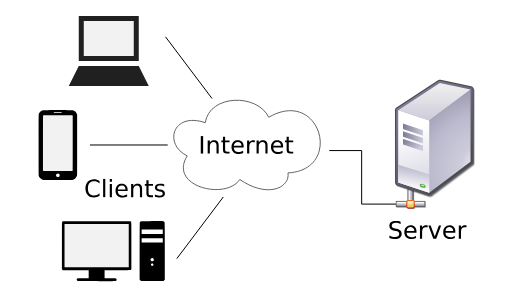
\includegraphics[width=120mm]{arch.png}}
		\caption{Arhitectură client-server}
\end{figure}

Caracteristica client-server descrie o relație de cooperare in aplicație. Componenta server expune o funcție sau un serviciu pentru unul sau mai mulți clienți. Clientul trebuie doar sa ințeleagă respunsul bazându-se pe un protocol prestabilit.

	\section{Sisteme distribuite}
Scopul programării distribuite este împarțirea funcționalitaților sau a modulelor spre a fi rulate in locații diferite. In proiectarea unui sistem distribuit trebuie tratate cazurile în care o componenta cade. Structura sistemului nu se cunoaste în avans, la fel ca infrastructura de comunicație. Orice componentă/calculator are doar o viziune limitata a întregului sistem. Modelul client-server este o implementare specifică a acestei paradigme.

	\section{Considerații IPC}
Inter-process communication se referă la mecanismele unui sistem de operare prin care pune la dispoziție proceselor pe care le găzduiește modalități de a comunica unele cu altele și de a trimite date de la unele la altele. În mod normal, aplicațiile pot folosi IPC sub forma modelului client-server, clientul cerând și serverul furnizând date. Multe aplicații pot fi și client și server, așa cum este de multe ori cazul in distributed computing. Metodele de implementare ale IPC sunt împarțite pe categorii bazate pe cerințe software (performanță sau modularitate), circumstanțe de sistem, etc. IPC este foarte important pentru procesul de proiectare a microkernelelor și nanokernlelelor. Microkernele reduc numarul de funcționalități pe care le expune kernelul. Acele funcționalități sunt obținute ulterior via IPC. Un microkernel folosește IPC mult mai intens față de un kernel monolitic convențional.

Există numeroase abordari și implementări pentru IPC:
\begin{itemize}
\item fișier pe disc
\item semnal
\item socket
\item Unix domain socket
\item coadă de mesaje
\item pipe
\item named pipe sau FIFO
\item etc
\end{itemize}

Sistemele POSIX, dar și Windows, includ majoritatea acestor mecanisme.

	\section{Nucleul sistemului de operare}
Kernelul este programul care stă la baza sistemului de operare și are control asupra intregului sistem. La majoritatea sistemelor de operare, nucleul este printre primele programe care se încarcă in memorie la start-up, imediat după bootloader. Este responsabil cu I/O, traducerea stream-urilor de date de la aplicații in instrucțiuni pentru procesor, arbitrează procese, alocă spațiu pentru utilizator și alte funcții de bază ale sistemului de operare. În mod normal, nucleul se incarcă intr-o zona specială și separată de memorie, protejată de accese ale aplicațiilor sau a componentelor mai puțin critice ale sistemului. Toate lucrurile critice sistemului au loc in kernel space, iar programele non-critice au loc in user space. Separând astfel user data de kernel data, se previne interferența și instabilitatea. Interfața nucleului este un nivel de abstractizare low-level. Apelurile de la procese către nucleu se numesc apeluri de sistem sau system calls.

\begin{figure}[h]
		\centering
			{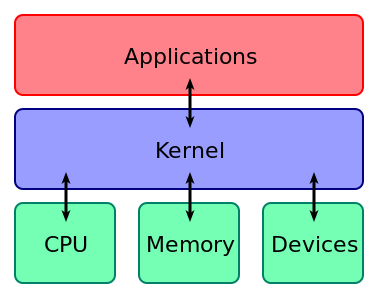
\includegraphics[width=100mm]{kernel.png}}
		\caption{Diagramă care ilustrează locul nucleului in stiva sistemului}
\end{figure}

Există diferite abordări de proiectare a nucleelor, printre care monolithic kernel, care ruleaza toate instrucțiunile de sistem in același spațiu de adresare sau microkernel, mai modular, care rulează multe din procesele critice in user space.

Scopul principal al nucleului este, deci, de a partaja resursele sistemului, incluzând:
\begin{itemize}
\item CPU
\item RAM
\item dispozitive I/O
\item management resurse
\item management memorie
\item management dispozitive
\item apeluri sistem
\end{itemize}

Nucleul Linux, folosit in proiect, este unul de tip monolitic, fiind extrem de rapid si versatil. Proiectarea unui kernel fiabil s-a dovedit dificilă și adesea foarte costisitoare ca timp. Folosirea unui kernel consacrat și fiabil și construirea sistemului peste acesta reprezintă un compromis optim de timp și resurse. Nucleul Linux este cel mai popular kernel monolitic Unix-like și pe baza lui s-a construit familia de sisteme de operare GNU/Linux, care conține mii de distribuții. Datorită capabilităților sale multi-CPU, nucleul Linux și-a consolidat poziția pe piața server si enterprise.


\chapter{Specificațiile proiectului}
	\section{Placa de dezvoltare gazdă - Raspberry Pi 3}
Probabil cea mai populara placa de dezvoltare cu microprocesor, Raspberry Pi 3 are următoarele specificații:
\begin{itemize}
\item procesor Broadcom BCM2837B0, Cortex-A53 (ARMv8) 64-bit SoC @ 1.4GHz
\item 1GB LPDDR2 SDRAM
\item placa de retea 2.4GHz and 5GHz IEEE 802.11 b/g/n/ac
\item Gigabit Ethernet over USB 2.0
\item extended 40 pin GPIO header
\item full-size HDMI
\item 4 porturi USB 2.0
\item slot de card micro SD
\item 5V @ 2.5A intrare alimentare
\end{itemize}

\begin{figure}
		\centering
			{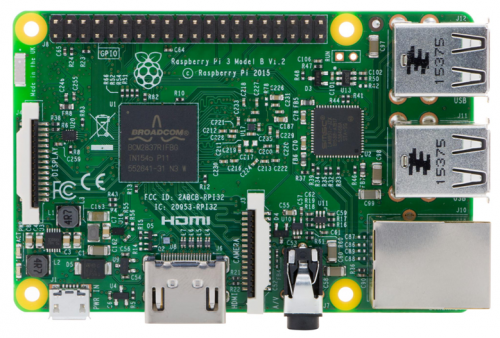
\includegraphics[width=80mm]{rpi.png}}
		\caption{Placa de dezvoltare Raspberry Pi 3}
\end{figure}

	\section{Workflow-ul normal pentru tipărire}
Un scenariu normal de printare prin CUPS presupune trimiterea pur și simplu a unui job de print către CUPS, iar acesta se va ocupa de restul. Un aspect important este abstractizarea imprimantelor în spatele 'cozilor' CUPS și se urmărește ca acest aspect sa rămână neschimbat. CUPS asignează fiecărei imprimante una sau mai multe 'cozi' (queues), iar acestea apar ca imprimante pe rețea pentru sistemele Unix (OSX, GNU/Linux, BSD, etc.).
Proiectul urmărește extragerea cat mai multor informații din procesul normal de printare CUPS, dar și menținerea modificărilor asupra CUPS la un nivel minim. O cerința importanta este ca workflow-ul normal de printare sa rămână neschimbat, iar modificările aduse pentru colectarea de date sa impacteze cat mai puțin platforma.

Modificările aduse CUPS trebuie sa se respecte următoarele cerințe:
\begin{itemize}
\item sa nu adauge overhead sistemului
\item sa nu expuna informatie proprietara Océ
\item sa nu modifice functionarea modulelor CUPS
\item să expună într-o manieră ușor de interceptat informațiile relevante
\item sa respecte licenta Apache v2.0 aferenta CUPS
\end{itemize}


\begin{figure}[h]
		\centering
			{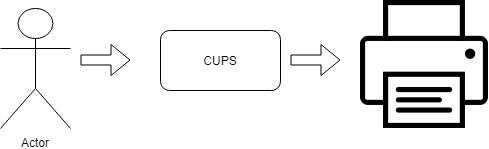
\includegraphics[width=110mm]{workflow.png}}
		\caption{Workflow-ul normal}
\end{figure}

	\section{Colectarea și stocarea datelor}
Modificările aduse CUPS urmăresc exclusiv colectarea datelor de imprimare și trimiterea lor către agregator. Colectarea datelor se face într-o maniera cat mai puțin invaziva, conform cerințelor anterior menționate. Se urmărește extragerea datelor spre a fi procesate, nu stocarea lor propriu zisa. Datele sunt transmise printr-un named pipe, prin urmare acestea nu părăsesc niciodată siguranța nucleului sistemului de operare. Lupa ce datele sunt recepționate și procesate de către agregator, acestea nu sunt salvate pe disc sau în alt mediu de stocare persistenta. Singurul loc în care datele persista este în Elasticsearch, dar este importanta mențiunea ca datele ajunse în Elasticsearch sunt deja procesate, iar în procesul de procesare pot fi eliminate orice informații nedorite.

Un alt criteriu important pe care proiectul a trebui sa îl respecte este respectarea confidențialității datelor. În niciun punct sistemul nu colectează date cu caracter personal, nici măcar numele utilizatorului, jobului sau mașina de pe care a fost trimis un print job. 


\chapter{Design și implementare}

	\section{Arhitectură high-level}

		\begin{figure}[h]
			\centering
				{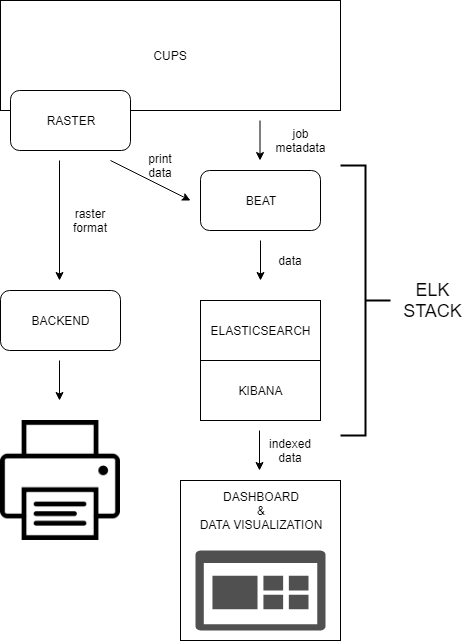
\includegraphics[width=110mm]{cups.png}}
			\caption{Arhitectura sistemului}
		\end{figure}

	\section{Componente software}
		\subsection{Sistemul de operare gazdă - BuruX}
Folosind CUPS ca backbone pentru sistem, s-a făcut evidenta nevoie folosirii unui sistem de operare Unix-like care sa îl găzduiască. Pe considerente de familiaritate s-a ales folosirea unui sistem de operare bazat pe nucleul Linux.
Nucleul Linux este un nucleu monolitic, adică lucrează în întregime separat de restul sistemului și în mod administrator. Driverele se pot încarcă în memoria de lucru la utilizare, de unde sunt șterse ulterior. Nucleul ofer facilități precum:
\begin{itemize}
\item multitasking
\item suport pentru memorie virtuala
\item suport avansat pentru TCP/IP
\item sistem de sunet
\item pana la 1 miliard de procese simultane
\item management avansat si eficient al memoriei
\item suport pentru sistem multi-procesor
\end{itemize}

Distribuția a fost compilata pentru arhitectura ARM, specifica procesorului Broadcom BCM2837 cu 4 nuclee ARM Cortex-A53, spre a fi instalata pe o placa Raspberry Pi 3. Procesorul și memoria de 1GB ale plăcii sunt mai mult decât suficiente pentru a rula sistemul de operare și componentele menționate mai sus. Versiunea de kernel folosita este 4.14, cu niște patch-uri suplimentare care sa permită folosirea modulelor Bluetooth și Wi-Fi ale plăcii. În testele efectuate, sistemul de operare este perfect stabil și consuma foarte puține resurse comparativ cu o distribuție de Linux full blown. Compilarea completa a sistemului de operare se face, pe o mașina relativ veche, în sub 25 minute. Nucleul linux este principala componenta a sistemului de operare GNU/Linux. Pentru use-case-ul de fata, am ales sa nu instalez un desktop environment sau interfața grafica pe sistem, pe considerente de reducere a resurselor consumate.
Distribuția de Linux folosita a fost compilata special pentru acest uz, drept urmare majoritatea funcțiilor au fost eliminate, rămânând doar cu cele strict esențiale pentru funcționarea CUPS:
\begin{itemize}
\item facilitati elementare de networking - Avahi
\item o selectie minimala de unelte si compilatoare - clang, golang
\item sistemul de printing CUPS cu dependentele aferente
\item functionalitate de remote access - SSH
\end{itemize}

Pentru compilare și aplicare de patch-uri a fost folosit Buildroot - o unealta care automatizează procesul de building al unui mediu Linux complet și bootabil, folosind cross-compilation pentru a putea servi multiple platforme. Buildroot își poate build-ui propriul toolchain, crea un root file system, compila o imagine de Linux kernel și genera un boot loader pentru sistemul dorit. Acesta funcționează pe baza unor fișiere de configurații, numite defconfigs, care conțin informații relevante pentru procesul de build (versiune de kernel, arhitectura, target file system, etc.). Sunt suportate mai multe biblioteci de C, printre care GNU C Library, uClibc și musl. Intern, Buildroot folosește Kconfig pentru sistemul de configurație, acesta oferind facilități precum o interfață cu meniu, ocuparea de dependente, opțiunea de 'Help' contextual. Întregul proces de build se construiește în jurul pachetelor descărcate automate în funcție de defconfig. Aceste pachete pot include aplicații, utilitati, biblioteci, etc. Rezultatul final este un root file system care poate fi copiat pe un mediu bootabil și folosit as-is. Buildroot face tot procesul de compilare, build și deployment ușor de înțeles și accesibil oricui.

Pe parcurs, a apărut problematica alegerii unui sistem de init. Buildroot pune la dispoziție implicit BusyBox - o implementare a unui program rudimentar de init, suficient pentru majoritatea aplicațiilor.
		\subsection[CUPS]{CUPS\\ {\normalsize Common UNIX Printing System}}
Apărut in 1999, CUPS este un sistem modular de printing open-source pentru sistemele de operare Unix-like. Acesta permite unui calculator sa se comporte ca un print server, devenind un host care accepta job-uri de la clienți, le procesează și le trimite către imprimante.
CUPS este format dintr-un spooler, un scheduler, un sistem de filtre care transforma datele dintr-un format în altul, și un sistem de backend-uri care realizează comunicarea cu imprimantele.

Workflow-ul standard CUPS este următorul: un job ajunge în scheduler, acesta îl trimite către unul sau mai multe filtre spre a fi convertit în alt format, apoi datele ajung într-un backend de unde sunt trimise spre printer. Sistemul folosește extensiv PostScript și rasterizarea datelor ca formate înțelese de imprimante.
			\subsubsection{Scheduler-ul CUPS}
Scheduler-ul CUPS implementează Internet Printing Protocol și oferă o interfață web-based pentru managementul imprimantelor, job-urilor, configurații server și documentație. Pentru accesarea funcționalităților de management și configurație, un utilizator trebuie sa se autentifice.
O alta parte foarte importanta a scheduler-ului este modulul de logging. Acesta înregistrează evenimente legate de acces, erori sau page log.
Alte module importante ale schedeuler-ului sunt: modulul MIME (multipurpose internet mail extensions), modulul PPD (PostScript printer description), modulul care se ocupa cu management-ul dispozitivelor disponibile în sistem.


			\subsubsection{Sistemul de filtre CUPS}
Sistemul de filtre al CUPS poate procesa o varietate de formate. Acesta convertește datele unui print-job într-un limbaj/format final printr-un sistem de filtre, folosind MIME types pentru identificarea formatelor.
Procesul de filtrare începe prin determinarea tipului de date de intrare, folosind MIME databases. Printre filtrele default ale CUPS se număra: raster to PCL, raster to ESC/P, raster to Dymo, raster to ZPL.
Inițial, am încercat modificare scheduler-ului, mai exact a modulului de logging, dar informațiile pe care le puteam obține din acesta erau insuficiente pentru cerințele proiectului, în modulul de logging fiind expuse numai date despre utilizatori, job-uri sau status. Considerând nevoia de a obține date despre pixeli, culoare, media, pagina, etc. s-a făcut necesara accesarea informațiilor disponibile în sistem de filtre al CUPS, mai exact în unitatea de raster. Lupa ce am identificat informațiile de care am nevoie, le-am trimis către exterior printr-un HTTP POST, apoi printr-un named pipe. Folosind un apel de sistem către comanda cURL pentru a trimite cererea HTTP către Beat, s-ar fi creat un număr de procese greu de controlat și care ar fi generat overhead pe care îl puteam evita. O a doua alternativa ar fi fost folosirea unei biblioteci, de exemplu libcurl, pentru a înlocui apelurile de sistem, dar aceasta alternativa ar fi introdus o dependenta suplimentara în CUPS, ceea ce ar fi făcut codul mai puțin portabil și ar fi încălcat una din cerințele inițiale ale proiectului. I final, am folosit un named pipe pentru transmiterea datelor, acesta fiind ușor de accesat și generând overhead minim, iar în plus, datele nu sunt expuse în rețea, aceasta interfața rezidând în kernelul sistemului de operare.


			\subsubsection{Backend-urile CUPS}
Backend-urile CUPS sunt folosite pentru a trimite datele către imprimante. CUPS pune la dispoziție multe backend-uri: paralel, serial, USB, cups-pdf, PDF virtual printing, JetDirect, LPD, SMB, etc.
		
		
		\subsection[Elastic Stack]{Elastic Stack\\ {\normalsize Beater - Elasticsearch - Kibana}}
Elastic Stack este o stiva de aplicații care permite extragerea, procesarea și vizualizarea datelor. În majoritatea cazurilor, acesta este găsit sub numele de ELK Stack (Elasticsearch - Logstash - Kibana). Pentru aceasta teza nu a fost folosit Logstash, fiind înlocuit cu un Elastic Beater ca unealta de colectare a datelor. Un Beat implementează interfața Beater și aduna date spre a le trimite către Kibana sau, în cazul de fata, Elasticsearch.


			\subsubsection{Beat}
Beat-urile au fost adăugate recent la stack-ul ELK. Un Beat are responsabilitatea sa colecteze date și sa le trimită spre procesare sau vizualizare. Acesta trebuie sa implementeze în Golang o interfață numita Beater interface, care conține metode de Start, Run și Stop. Aceasta lucrare folosește un Beat pentru a primi date de la raster-ul, raster care face parte din sistemul de filtre menționat anterior. Beat-ul primește raster data, face operații de procesare și sanitization minimale, apoi trimite datele către Elasticsearch. În  implementările convenționale de Beat, datele sunt transmise la intervale periodice de timp către Elasticsearch sau Kibana. Implementarea Beat-ului din aceasta lucrare trimite date către Elasticsearch atunci când primește informații noi de la raster. cBeat (Beater-ul implementat pentru aceasta lucrare) următoarele componente principale:
\begin{outline}
\1 {\large Metodele interfetei Beater}
	\2
	\textbf{metoda Run}
		\3 contine bucla principala a aplicatiei
		\3 in interiorul buclei se transmit evenimente catre restul ELK stack
		\3 un eveniment este trimis encodat ca JSON catre Elasticsearch
		\3 mai jos este exemplificata metoda Run din exemplul oferit de Elastic
		\3 se observa cum evenimentele sunt trimise la intervale periodice de timp
\begin{lstlisting}[caption={exemplu metoda Run - golang},captionpos=b]
func (bt *Countbeat) Run(b *beat.Beat) error {
logp.Info("countbeat is running! Hit CTRL-C to stop it.")

bt.client = b.Publisher.Connect()
ticker := time.NewTicker(bt.config.Period)
counter := 1
for {
select {
case <-bt.done:
return nil
case <-ticker.C:
}

event := common.MapStr{
"@timestamp": common.Time(time.Now()),
"type": b.Name,
"counter": counter,
}
bt.client.PublishEvent(event)
logp.Info("Event sent")
counter++
}
}
\end{lstlisting}

	\2
	\textbf{metoda Stop}
		\3 este chemata atunci când Beat-ul e semnalat sa se oprească
		\3 mai jos este exemplificata metoda Stop
\begin{lstlisting}[caption={exemplu metoda Stop - golang},captionpos=b]
func (bt *Countbeat) Stop() {
bt.client.Close()
close(bt.done)
}
\end{lstlisting}
\1 {\large Recepționarea datelor din CUPS}
	\2 citirea din named pipe a evenimentelor se face prin deschiderea FIFO-ului ca orice alt fișier de pe disk, folosind modulul os al Golang
\begin{lstlisting}[caption={deschidere named pipe - golang},captionpos=b]
pipePath = "/tmp/cupsbeat"
if p, err = os.Open(pipePath); os.IsNotExist(err) {
log.Fatalf("Named pipe '\%s' does not exist", pipePath)
} else if os.IsPermission(err) {
log.Fatalf("Insufficient permissions to read named pipe '\%s': \%s", pipePath, err)
} else if err != nil {
log.Fatalf("Error while opening named pipe '\%s': \%s", pipePath, err)
}
defer p.Close()
\end{lstlisting}

	\2 FIFO-ului i s-a adăugat un mecanism de watch care ne notifica atunci când s-a efectuat orice scriere în pipe
\begin{lstlisting}[caption={watch pentru named pipe - golang},captionpos=b]
c := make(chan notify.EventInfo, MAX_CONCURRENT_WRITERS)
notify.Watch(pipePath, c, notify.Write|notify.Remove)
\end{lstlisting}

	\2 funcția care supraveghează pipe-ul a fost lansata într-o go rutina în metoda Run
\begin{lstlisting}[caption={apel readPipe in go routina separata - golang},captionpos=b]
go func(){
	readPipe()
}()
\end{lstlisting}
	\2 ca mecanism IPC s-a folosit un go channel intre green thread-ul care citește din pipe și cel al metodei principale
\begin{lstlisting}[caption={instantiere canal - golang},captionpos=b]
var messageQueue = make(chan Message_s_t)
\end{lstlisting}

\1 {\large Generarea structurilor necesare prelucrării datelor}
	\2 pe baza enum-urilor definite în CUPS se urmărește generarea unor structuri de date echivalente în limbajul Go
\begin{lstlisting}[caption={exemplu enum CUPS - C},captionpos=b]
typedef enum cups_adv_e			/**** AdvanceMedia attribute values ****/
{
CUPS_ADVANCE_NONE = 0,		/* Never advance the roll */
CUPS_ADVANCE_FILE = 1,		/* Advance the roll after this file */
CUPS_ADVANCE_JOB = 2,			/* Advance the roll after this job */
CUPS_ADVANCE_SET = 3,			/* Advance the roll after this set */
CUPS_ADVANCE_PAGE = 4			/* Advance the roll after this page */
} cups_adv_t;

\end{lstlisting}
	\2 pentru transmiterea eficienta a datelor, se păstrează encodarea diferitor opțiuni de tipărire în numere întregi
	\2 generarea de cod Go din fișierele header care conțin structurile CUPS presupune parcurgerea lor
	\2 rezultatul final trebuie sa fie un fișier .go compilabil care conține structurile echivalente
	\2 s-a folosit un algoritm similar cu un automate care parcurge fișierul
	\2 automatul salvează fiecare intrare într-un dicționar de dicționare de șiruri de caractere
\begin{lstlisting}[caption={instantiere dictionar - golang},captionpos=b]
var maps = make(map[string]map[string]string)
\end{lstlisting}
	\2 fiecare intrare corespunde unui enum, cu dicționarul corespunzător
	\2 intrările din dicționarul corespunzător reprezinta perechile de întregi - șir de caractere
	\2 întregul modul de generare de cod a fost scris în limbajul Go
\begin{lstlisting}[caption={structuri de date pentru generator/procesor date - golang},captionpos=b]
type HWResolution_t struct {
	Hr1 int
	Hr2 int
}

type ImaginBoundingBox_t struct {
	Ibb1 int
	Ibb2 int
	Ibb3 int
	Ibb4 int
}

type PageSize_t struct {
	Ps1 int
	Ps2 int
}

type Message_t struct{
	CutMedia int
	Duplex int
	HWResolution HWResolution_t
	ImagingBoundingBox ImaginBoundingBox_t
	InsertSheet int
	Orientation int
	NumCopies int
	PageSize PageSize_t
	Tumble int
	CupsWidth int
	CupsHeight int
	CupsBitsPerColor int
	CupsBitsPerPixel int
	CupsColorOrder int
	CupsColorSpace int
	CupsNumColors int
}

type Message_s_t struct{
	CutMedia string
	Duplex int
	HWResolution HWResolution_t
	ImagingBoundingBox ImaginBoundingBox_t
	InsertSheet int
	Orientation string
	NumCopies int
	PageSize PageSize_t
	Tumble int
	CupsWidth int
	CupsHeight int
	CupsBitsPerColor int
	CupsBitsPerPixel int
	CupsColorOrder string
	CupsColorSpace string
	CupsNumColors int
}
\end{lstlisting}

\1 {\large Prelucrarea datelor}
	\2 la compilare, se populează structurile menționate la punctul anterior pe baza header-ului CUPS
	\2 atunci când se recepționează un eveniment, avesta ajunge in Beat sub forma de string
	\2 evenimentul este procesat pe baza dicționarelor, întregii fiind înlocuiți cu stringuri
	\2 după prelucrare, evenimentul este serializat ca JSON și este trimis către Elasticsearch

\begin{lstlisting}[caption={functia pentru procesarea mesajelor - golang},captionpos=b]
func processMsg(msg string) Message_s_t{
	var maps = cups_itf.Maps
	fmt.Println(maps["Duplex"]["0"])
	logp.Info("PROCESSING STRING:")
	logp.Info(msg)
	var message Message_t
	var message_s Message_s_t
	if isJSON(msg){
		logp.Info("VALID JSON")
		json.Unmarshal([]byte(msg), &message)
		message_s.CutMedia = maps["CutMedia"][strconv.Itoa(message.CutMedia)]
		message_s.Duplex = message_s.Duplex
		message_s.HWResolution = message.HWResolution
		message_s.ImagingBoundingBox = message.ImagingBoundingBox
		message_s.InsertSheet = message.InsertSheet
		message_s.Orientation = maps["Orientation"][strconv.Itoa(message.Orientation)]
		message_s.NumCopies = message.NumCopies
		message_s.PageSize = message.PageSize
		message_s.Tumble = message.Tumble
		message_s.CupsWidth = message.CupsWidth
		message_s.CupsHeight = message.CupsHeight
		message_s.CupsBitsPerColor = message.CupsBitsPerColor
		message_s.CupsBitsPerPixel = message.CupsBitsPerPixel
		message_s.CupsColorOrder = maps["cupsColorOrder"][strconv.Itoa(message.CupsColorOrder)]
		message_s.CupsColorSpace = maps["cupsColorSpace"][strconv.Itoa(message.CupsColorSpace)]
		message_s.CupsNumColors = message.CupsNumColors
		logp.Info("CREATED NEW STRUCT")
	}
	return message_s
}
\end{lstlisting}
\end{outline}


			\subsubsection{Elasticsearch}
Elasticsearch este un motor de căutare bazat pe Apache Lucene. Oferă clienți disponibili în majoritatea tehnologiilor și este cel mai popular motor de căutare enterprise. Beneficiile Elasticsearch includ: căutare foarte scalabila, aproape real-time, suportul mai multor clienți, platforma distribuita. Este considerat de multi backbone-ul stack-ului ELK. Informațiile extrase de Beat ajung în Elasticsearch, iar acesta cauta tipare și indexează datele spre a le trimite către Kibana.


			\subsubsection{Kibana}
Kibana este un plugin open-source pentru vizualizare de data, care pune la dispoziție capabilități de vizualizare ale elementelor indexate într-un cluster Elasticsearch. Un utilizator poate construi diferite tipuri de grafice bazate pe datele indexate de Elasticsearch, iar pe baza acestor grafice se pot construi dashboard-uri configurabile. Kibana preia datele indexat de la Elastisearch și le folosește la generarea de grafice și vizualizări relevante pentru utilizator.

Stat Elasticsearch, cat și Kibana sunt hostate pe o mașina (Debian) în cloud pe platforma Scaleway. Mașina are o configurație minimala, stack-ul fiind unul robust și eficient nu are nevoie de multe resurse. Administrarea mașinii se face strict prin SSH, iar interfața web Kibana este expusa spre exterior. Prin intermediul aplicației web se face și configurarea graficelor și dashboard-ului Kibana. Pe mașina host este instalat nginx care redirectează orice acces HTTP către portul Kibana (9300).
	\section{Build și deployment}
	Build-ul CUPS presupune compilarea fișierelor C din proiect și linkeditarea corespunzatoare. Apple pune la dispoziție un Makefile pentru build. Build-ul Beat se face prin compilarea fișierelor Go aferente, si el avand un Makefile.
	Deployment-ul CUPS se face local, pe mașina de unde se urmărește extragerea informațiilor. Acest lucru se realizează prin copiere binarelor în locația corespunzătoare sau prin instalarea unui pachet .deb, .rpm, etc. generat pentru fiecare platforma în parte.
	Kibana și Elasticsearch sunt deployed pe o masina in cloud, pe platforma Scaleway. Pe mașina este instalat nginx, care oferă capabilități de proxy si routing elementare.
	\begin{figure}
		\centering
		{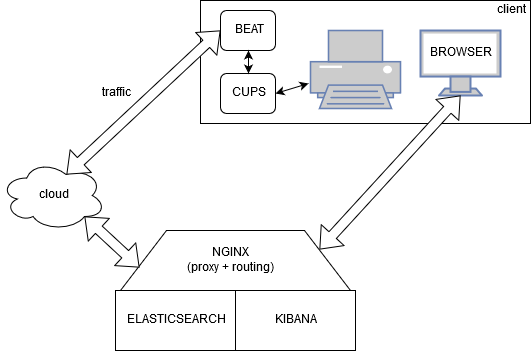
\includegraphics[width=130mm]{cups-cloud.png}}
	\caption{comunicarea CUPS - Beat - Elasticsearch - Kibana - Utilizator}
	\end{figure}	
	Dacă se introduce adresa mașinii într-un browser, nginx va redirecta direct catre Kibana.
	\begin{figure}
		\centering
		{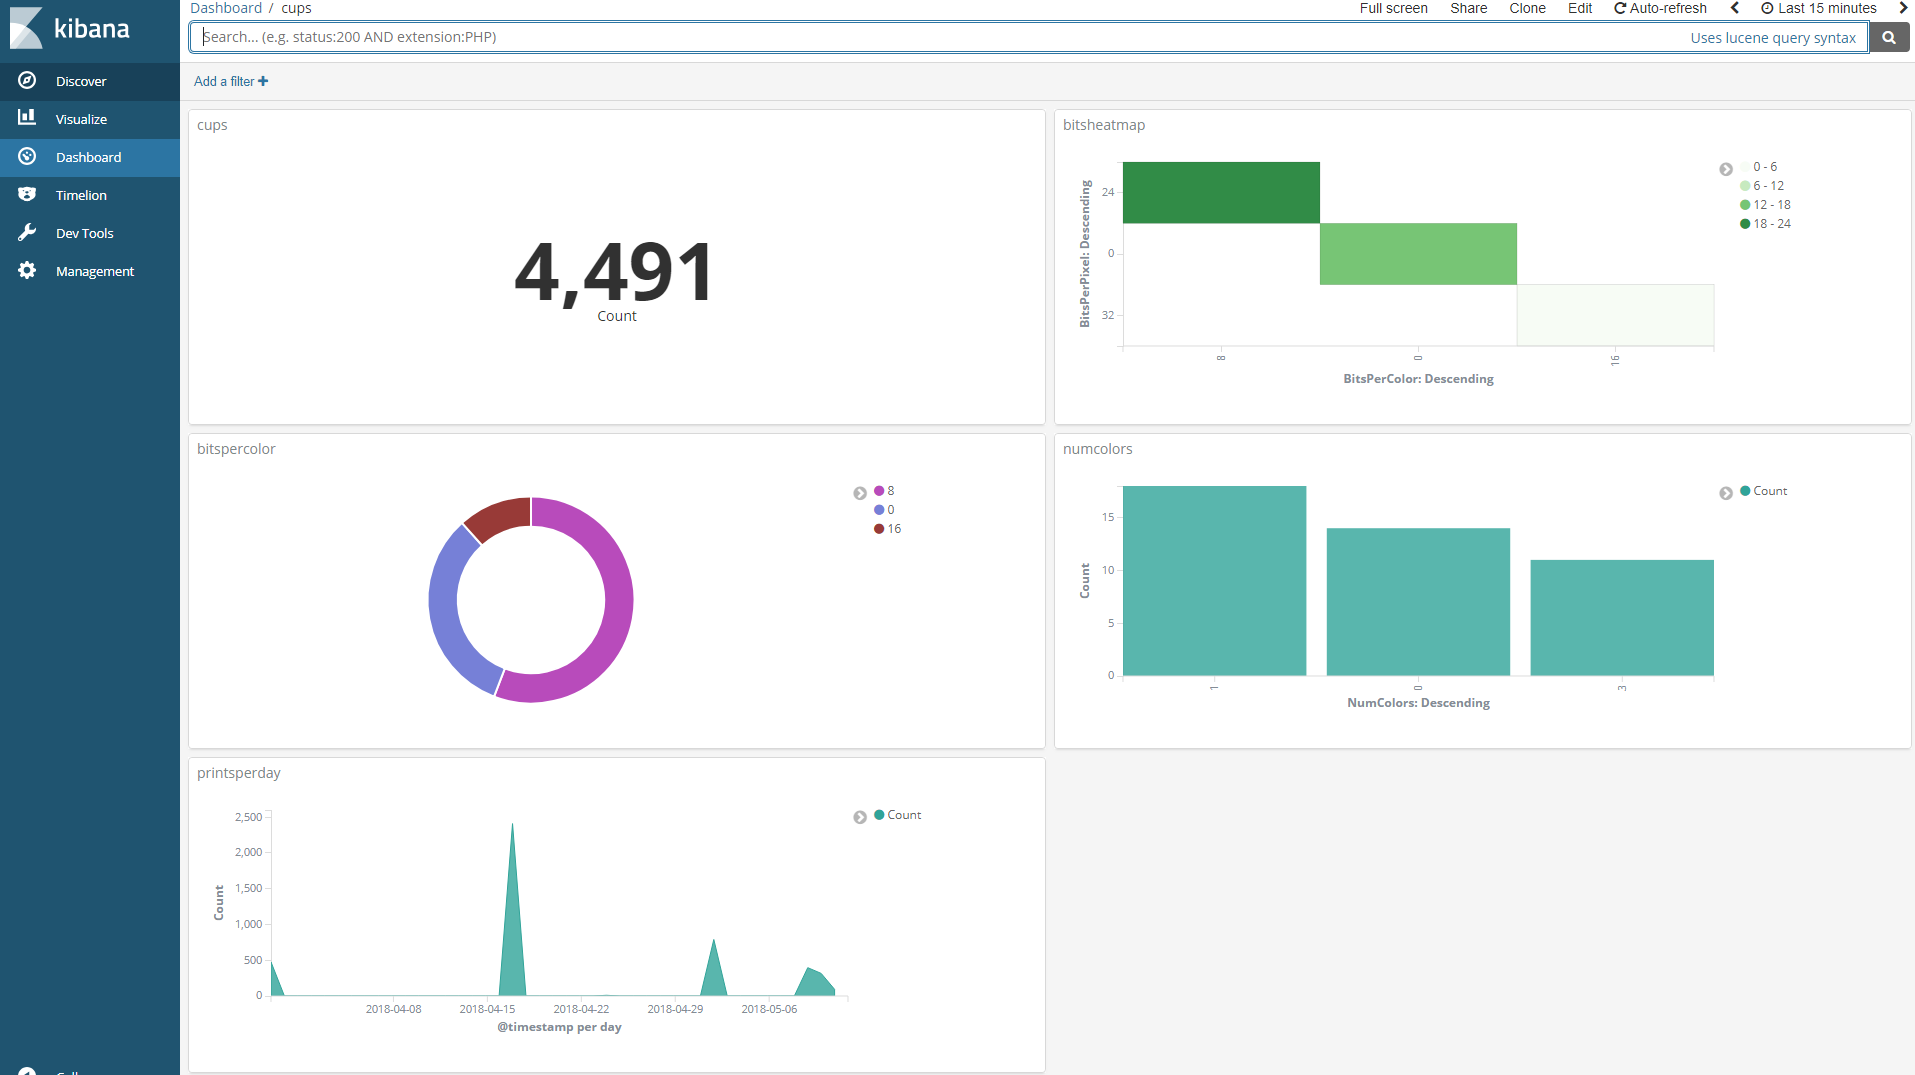
\includegraphics[width=160mm]{kibana-dashboard.png}}
		\caption{dashboard-ul Kibana intr-o fereastra de browser}
	\end{figure}
	Fiecare grafic din dashboard este configurabil. Configurația include tipul de metrici folosite, tipul de metoda de agregare, axele, cate metrici sunt folosite, cate și care câmpuri sunt folosite, etc.
	\begin{figure}
		\centering
		{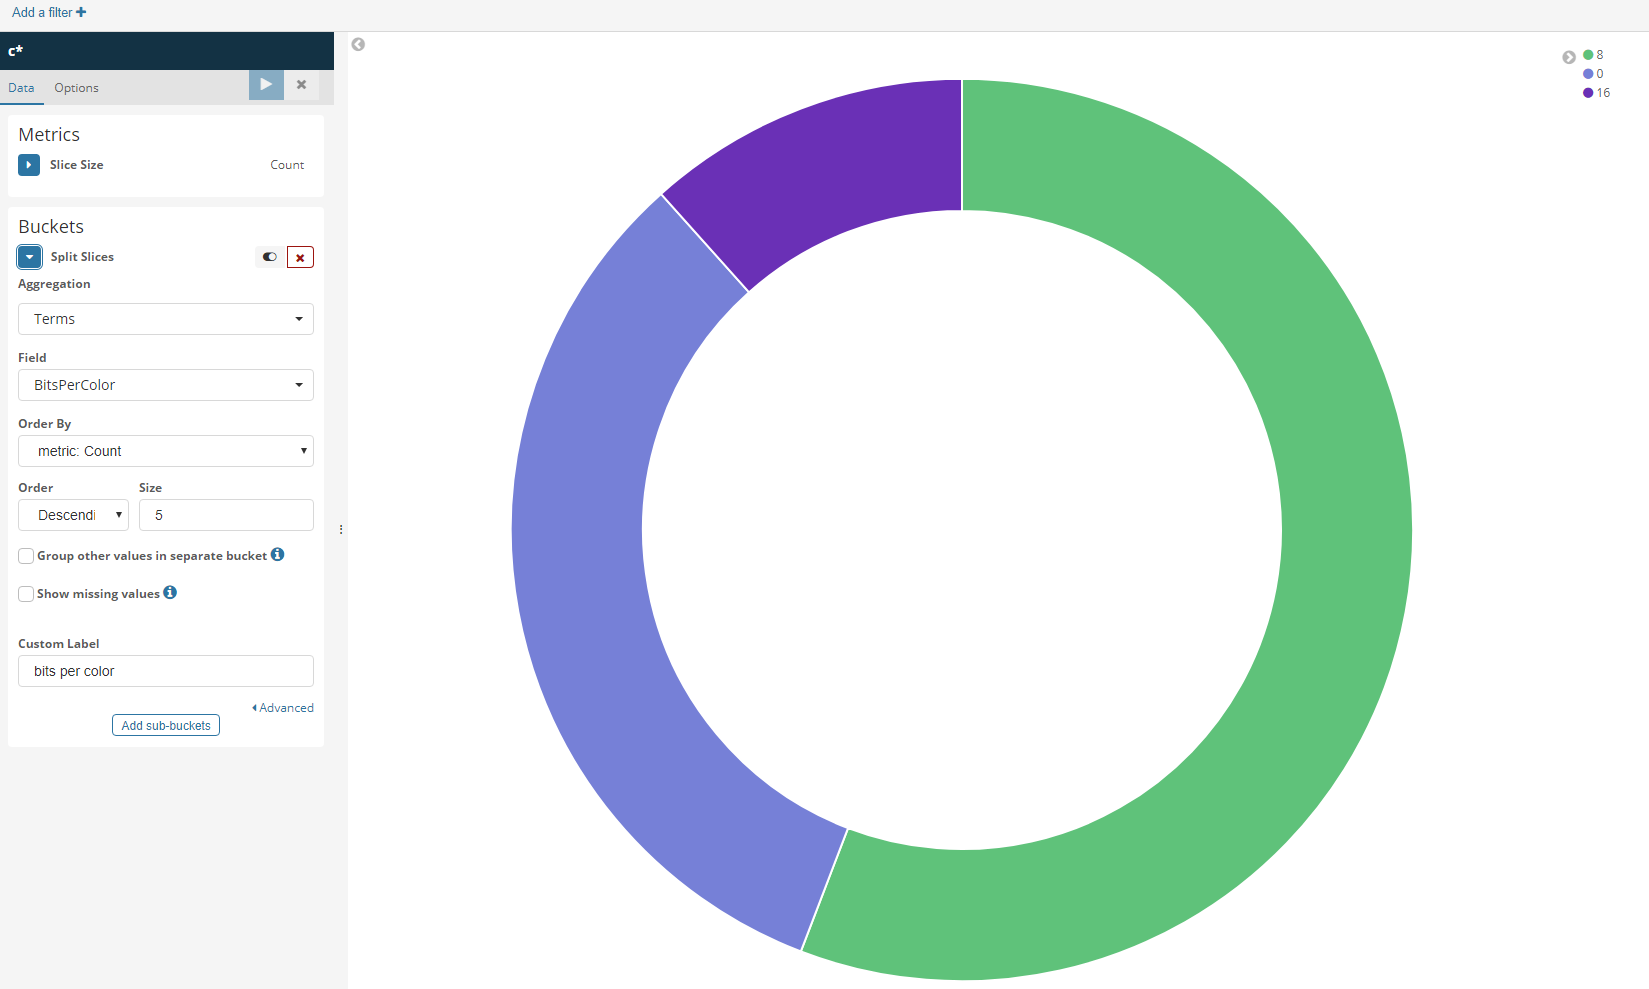
\includegraphics[width=160mm]{kibana-chart-config.png}}
		\caption{dashboard-ul Kibana intr-o fereastra de browser}
	\end{figure}
	\begin{figure}
		\centering
		{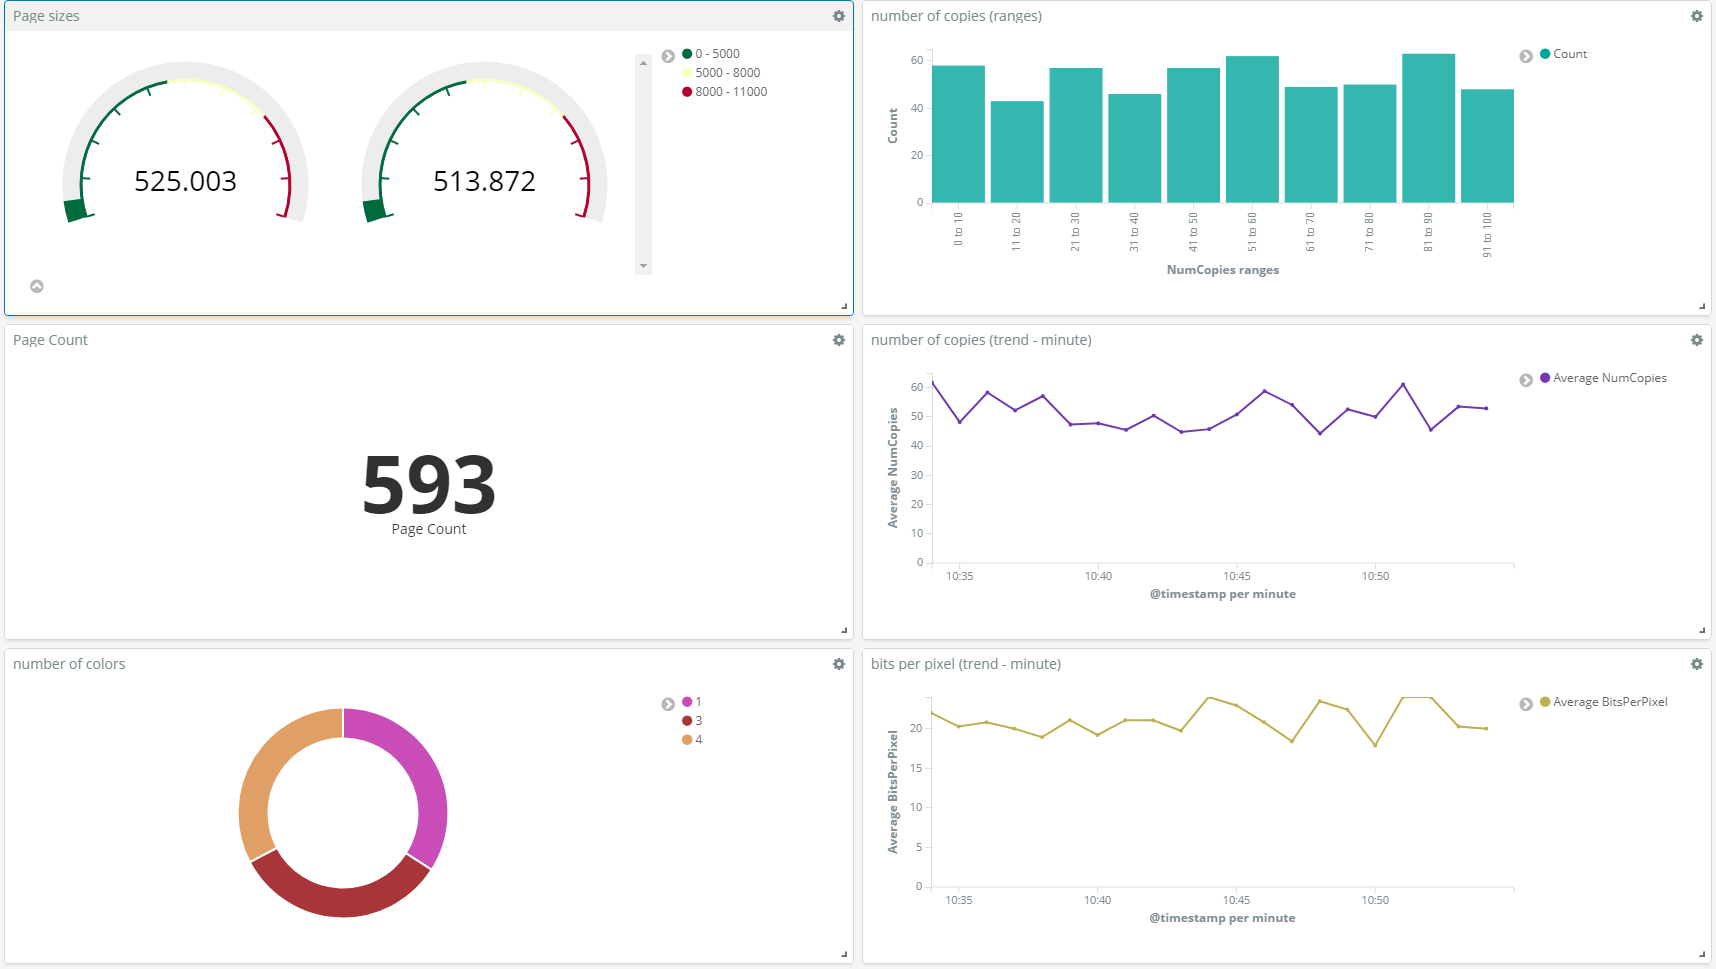
\includegraphics[width=160mm]{dashboard.png}}
		\caption{exemple de grafice in Kibana; de la dreapta la stanga, de sus in jos: page size, intervale de numere de copii, page count, trend in timp cu numere de copii, pie chart cu numar de culor si trend in timp cu bits per pixel}
	\end{figure}
	\subsection{Stubbing}
	Dat fiind ca datele de tipărire care se pot colecta intr-un timp scurt sunt limitate, s-a decis implementarea unui program care să simuleze tipărirea prin generarea de tichete JSON asemănătoare celor trimise de CUPS, dar cu valori arbitrare pentru fiecare câmp, evident cu constraint-urile aferente. Implementarea a fost făcută in Python3. Programul parcurge enum-urile C ale CUPS menționate anterior si generează pe baza lor un JSON. Acesta este trimis către Beat, spre a fi prelucrat ca orice tichet venit din CUPS. Stub-ul ajuta la colectarea de date și exemplificarea funcționalității dashboard-ului Kibana. Generatorul de tichete este paremetrizat cu constraint-uri si valori rezonabile pentru fiecare camp din JSON.  
\begin{lstlisting}[caption={cazul general dupa care se populeaza tichetul - Pyton},captionpos=b]
# CONSTANTS
class Constraints(object):
    def __init__(self):
        self.cupsBitsPerColor = [8, 16, 32]
        self.cupsBitsPerPixel = [8, 24, 32]
        self.cupsColorOrder = [0, 1, 2]
        self.cupsColorSpace = [0, 1, 2, 3, 4, 5]
        self.CutMedia = [0, 1, 2, 3, 4]
        self.Duplex = [0]
        self.HW_RES_MAX = 8096
        self.IBB_MAX = 1024
        self.InsetSheet = [0]
        self.cupsNumColors = [1, 3, 4]
        self.NUM_COPIES_MAX = 100
        self.Orientation = [0, 1, 2 , 3]
        self.PAGE_SIZE_MAX = 8096
        self.Tumble = [0]
        self.CUPS_HEIGHT_MAX = 1024
        self.CUPS_WIDTH_MAX = 1024

const = Constraints()

def randomize(x):
    return randint(0,x)

class Blank(object):
    pass

special = ['HW_RES_MAX', 'IBB_MAX', 'NUM_COPIES_MAX', 'PAGE_SIZE_MAX', 'CUPS_HEIGHT_MAX', 'CUPS_WIDTH_MAX']

def get_populated_class():
    _json = Blank()
    fields = const.__dict__
    for k in fields:
        if k in special:
            pass
        else:
            setattr(_json, k, fields[k][randomize(len(fields[k])-1)])
\end{lstlisting}
În cazurile speciale, câmpurile sunt adaugate individual, unul câte unul. Aceste câmpuri sunt cele desemnate de membrii listei 'special' definite mai sus.
\begin{lstlisting}[caption={cazurile speciale, tratate individual - Python},captionpos=b]
# set HWResolution        
    res = Blank()
    setattr(res, 'hr1', randomize(const.HW_RES_MAX))
    setattr(res, 'hr2', randomize(const.HW_RES_MAX))
    setattr(_json, 'HWResolution', res.__dict__)

    # set ImagingBoundingBox
    ibb = Blank()
    setattr(ibb, 'ibb1', 0)
    setattr(ibb, 'ibb2', 0)
    setattr(ibb, 'ibb3', randomize(const.IBB_MAX))
    setattr(ibb, 'ibb4', randomize(const.IBB_MAX))
    setattr(_json, 'ImagingBoundingBox', ibb.__dict__)

    # set NumCopies
    setattr(_json, 'NumCopies', randomize(const.NUM_COPIES_MAX))

    # set PageSize
    ps = Blank()
    setattr(ps, 'ps1', randomize(const.PAGE_SIZE_MAX))
    setattr(ps, 'ps2', randomize(const.PAGE_SIZE_MAX))
    setattr(_json, 'PageSize', ps.__dict__)

    # set cupsHeight
    setattr(_json, 'cupsHeight', randomize(const.CUPS_HEIGHT_MAX))

    # set cupsWidth
    setattr(_json, 'cupsWidth', randomize(const.CUPS_WIDTH_MAX))
\end{lstlisting}
\begin{lstlisting}[caption={exemplu de output pentru programul de mai sus - JSON},captionpos=b]
{  
   "HWResolution":{  
      "hr1":3272,
      "hr2":670
   },
   "InsetSheet":0,
   "PageSize":{  
      "ps2":361,
      "ps1":6210
   },
   "CutMedia":2,
   "Orientation":3,
   "cupsColorOrder":1,
   "Tumble":0,
   "Duplex":0,
   "ImagingBoundingBox":{  
      "ibb4":819,
      "ibb3":863,
      "ibb2":0,
      "ibb1":0
   },
   "cupsBitsPerColor":8,
   "cupsWidth":736,
   "cupsHeight":163,
   "NumCopies":43,
   "cupsBitsPerPixel":24,
   "cupsNumColors":3,
   "cupsColorSpace":1
}
\end{lstlisting}
Tichetul este citit de Beat, iar valorile numerice ale câmpurilor sunt traduse în siruri de caractere corespunzatoare din enum-urile CUPS. 
Această abordare permite inclusiv testarea infrastructurii de transmitere si colectare de date.

	\subsection{Limbajul de interogare Lucene}
O interogare este descompusă sintactic in termeni si operatori. Termenii, la rândul lor, se impart in termeni simplii si fraze. Un termen simplu este un cuvânt, iar o frază este un grup de cuvinte. Mai mulți termeni pot fi combinați folosind operatori pentru a forma o interogare mai complexă. Analizor folosit pentru indexare se va folosi de termeni si fraze.

	\subsubsection{Câmpuri}
Lucene suportă date sub forma câmpurilor. Atunci cand se efectuează o interogare, sunt specificate câmpuri sau se folosesc câmpuri implicite. Numele câmpurilor sunt specifice fiecărei implementări. Pentru a căuta după un câmp se va folosi numele câmpului urmat de ":", apoi valoarea.
\begin{lstlisting}[caption={exemplu de căutare după câmpuri - Lucene query},captionpos=b]
title:"The Right Way" AND text:go
\end{lstlisting}

 	\subsubsection{Căutări wildcard}
Lucene suportă wildcards cu unul sai mai multe caractere în căutări.
\begin{itemize}
\item pentru căutare wildcard cu un singur caracter se va folosi simbolul "?"
\begin{lstlisting}[caption={căutare wildcard cu un singur caracter - Lucene query},captionpos=b]
te?t
\end{lstlisting}
\item pentru căutare wildcard multi-caracter se va folosi simbolul "*"
\begin{lstlisting}[caption={căutare wildcardmulti-caracter - Lucene query},captionpos=b]
te*t
\end{lstlisting}
\end{itemize}

	\subsubsection{Căutări fuzzy}
Sunt suportate căutările fuzzy bazate pe algoritmii Levenshtein Distance sau Edit Distance. Pentru a efectua o căutare fuzzy se va folosi simbolul "~" la finalulul unui termen. După Lucene 1.9 a fost adăugat un parametru suplimentare cu valoare între 0-1 care reprezinta similitudinile cu termenul căutat, pe o scara de la 0 la 1. Implicit se foloseste 0.5.
\begin{lstlisting}[caption={căutare fuzzy - Lucene query},captionpos=b]
test~0.9
\end{lstlisting}

	\subsubsection{Căutări pe intervale}
Permit găsirea acelor intrări care satisfac o condiție de genul A mai mic decat x mai mic decat B. Pentru interval inchis, deschis se folosesc acolade, repsectiv paranteze drepte.
\begin{lstlisting}[caption={căutari pe intervale - Lucene query},captionpos=b]
mod_date:[20020101 TO 20030101]

title:{Aida TO Carmen}
\end{lstlisting}

	\subsubsection{Elevarea relevanței unui termen}
Lucene permite ridicarea relevanței unui termen folosind operatorul special urmat de nivelul dorit. Cu cat nivelul este mai mare, cu atata termenul va fi mai relevant in interogare.
\begin{lstlisting}[caption={elevarea relevanței - Lucene query},captionpos=b]
"jakarta apache"^4 "Apache Lucene"
\end{lstlisting}

	\subsubsection{Operatori}
Operatorul implicit pentru conjuncție este SAU. Alți operatori sunt: SI, +, NOT, -.

% add this later on
\iffalse
\begin{figure}[h]
	\centering
		{
\includegraphics[width=100mm]{queries1.png}}
	\caption{Bara de căutare din Kibana (sus); două filtre aplicate (jos)}
\end{figure}
\fi

	\subsection{Limbajul de interogare Elasticsearch}

Kibana acceptă atât interogări Lucene, cât si interogări Elasticsearch. Oirce interogare Elasticsearch este scrisă sub forma unui JSON. Câmpul query din obiect desemnează tipul interogării.
 
\begin{lstlisting}[caption={exemplu interogare Elasticsearch - JSON},captionpos=b]
GET /bank/_search
{
  "query": {
    "bool": {
      "must": { "match_all": {} },
      "filter": {
        "range": {
          "balance": {
            "gte": 20000,
            "lte": 30000
          }
        }
      }
    }
  }
}
\end{lstlisting}

Interogarea din listing-ul de mai sus va returna toate conturile cu balance cuprins între 20000 si 30000. Se observă cum interogarea conține un {\textbf{\textit{match\_all}}} si un \textbf{\textit{range}}, ambele indicând tipuri de interogări.

Implicit, interogările returnează documentul JSON întreg ca parte a câmpului {\textbf{\textit{\_source}}. Dacă se dorete ca documentul să nu fie returnat, putem cere doar anumite câmpuri din obiect. Peste o interogare se pot aplica filtre si agregări. Elasticsearch este un produs atât simplu cât si complex. În general se foloseste împreuna cu un RESTful API.

	\subsection{Platforma Scaleway}
Pentru deployment s-a ales platforma Scaleway pe considerente practice si economice. Ea oferă performanțe similare platformelor mainstream la o fracțiune din preț. Scaleway foloseste masini ARM-based. Principalul avantaj față de alte platforme este că pornind de la pachetul de bază, toate includ stocare SSD, cu opțiune pentru NVMe SSD. Scaleway ofera root access complet pe un server dedicat. Performanțele sunt constante si predictibile, spre deosebire de servere virtuale. Platforma oferă flexibilitate pentru plata serviciilor, taxarea fiind făcută dinamic în funcție de timpul folosit. Pe lângă asta, Scaleway este printre singurele companii mari de hosting europene, având servere in Amsterdam si Paris. Latența din Timisoara este de sub 40 ms. Administrarea se face printr-o platforma web.
\begin{figure}[h]
	\centering
		{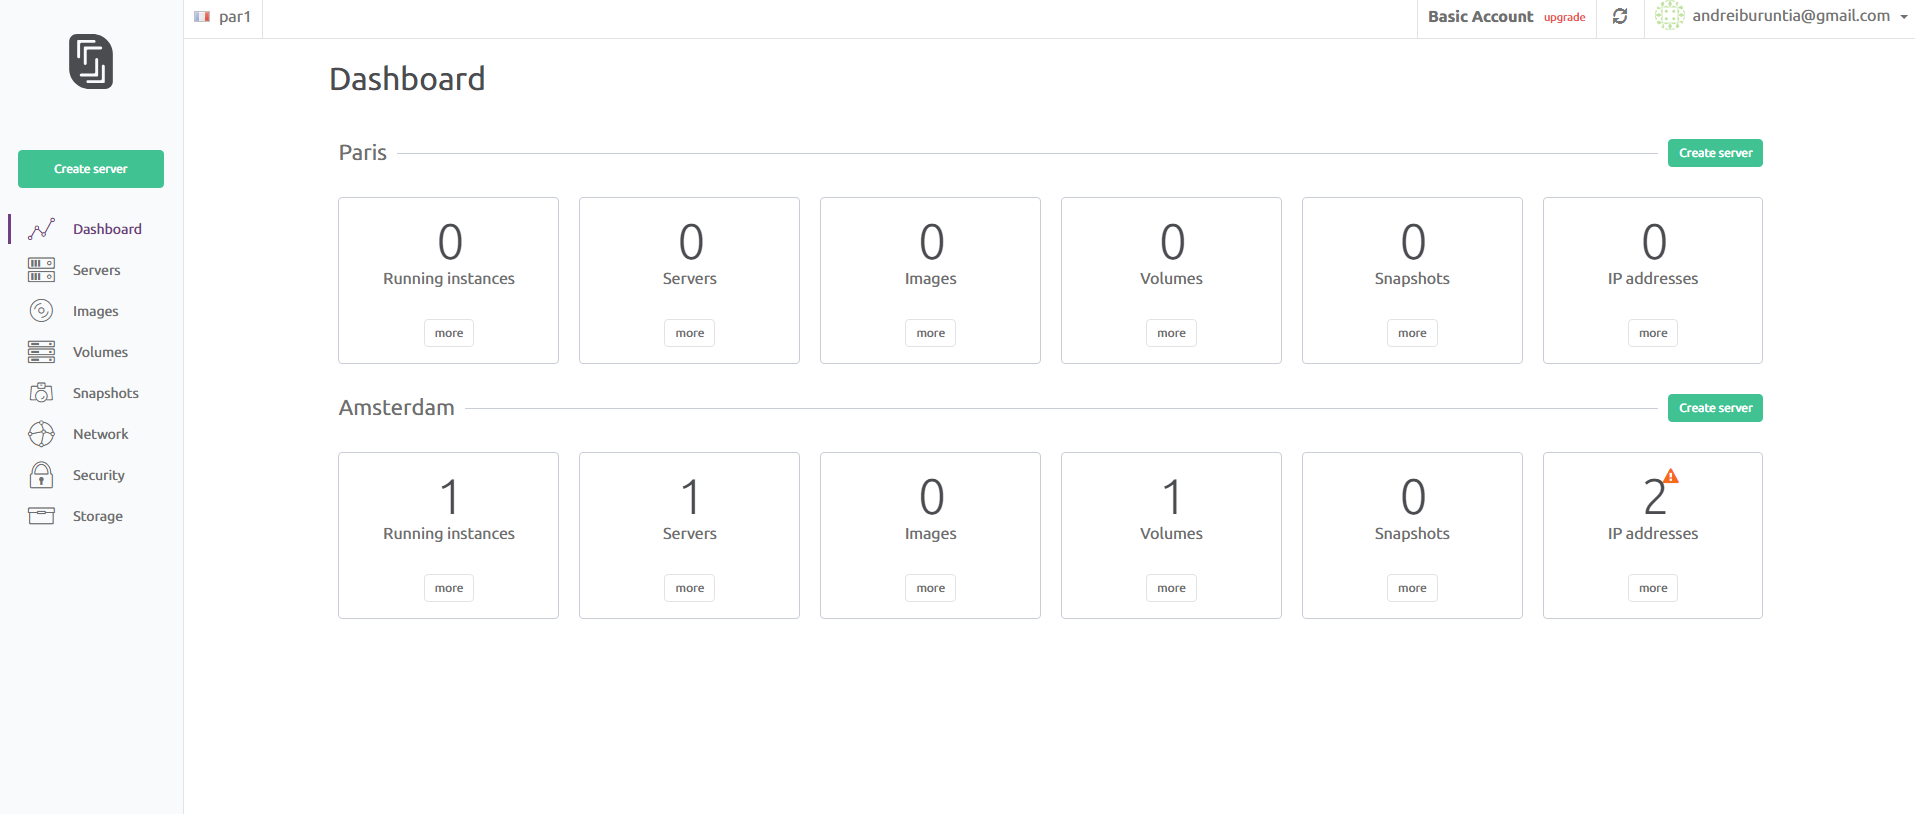
\includegraphics[width=170mm]{scaleway1.png}}
	\caption{Dashboard-ul Scaleway}
\end{figure}
\begin{figure}[h]
	\centering
		{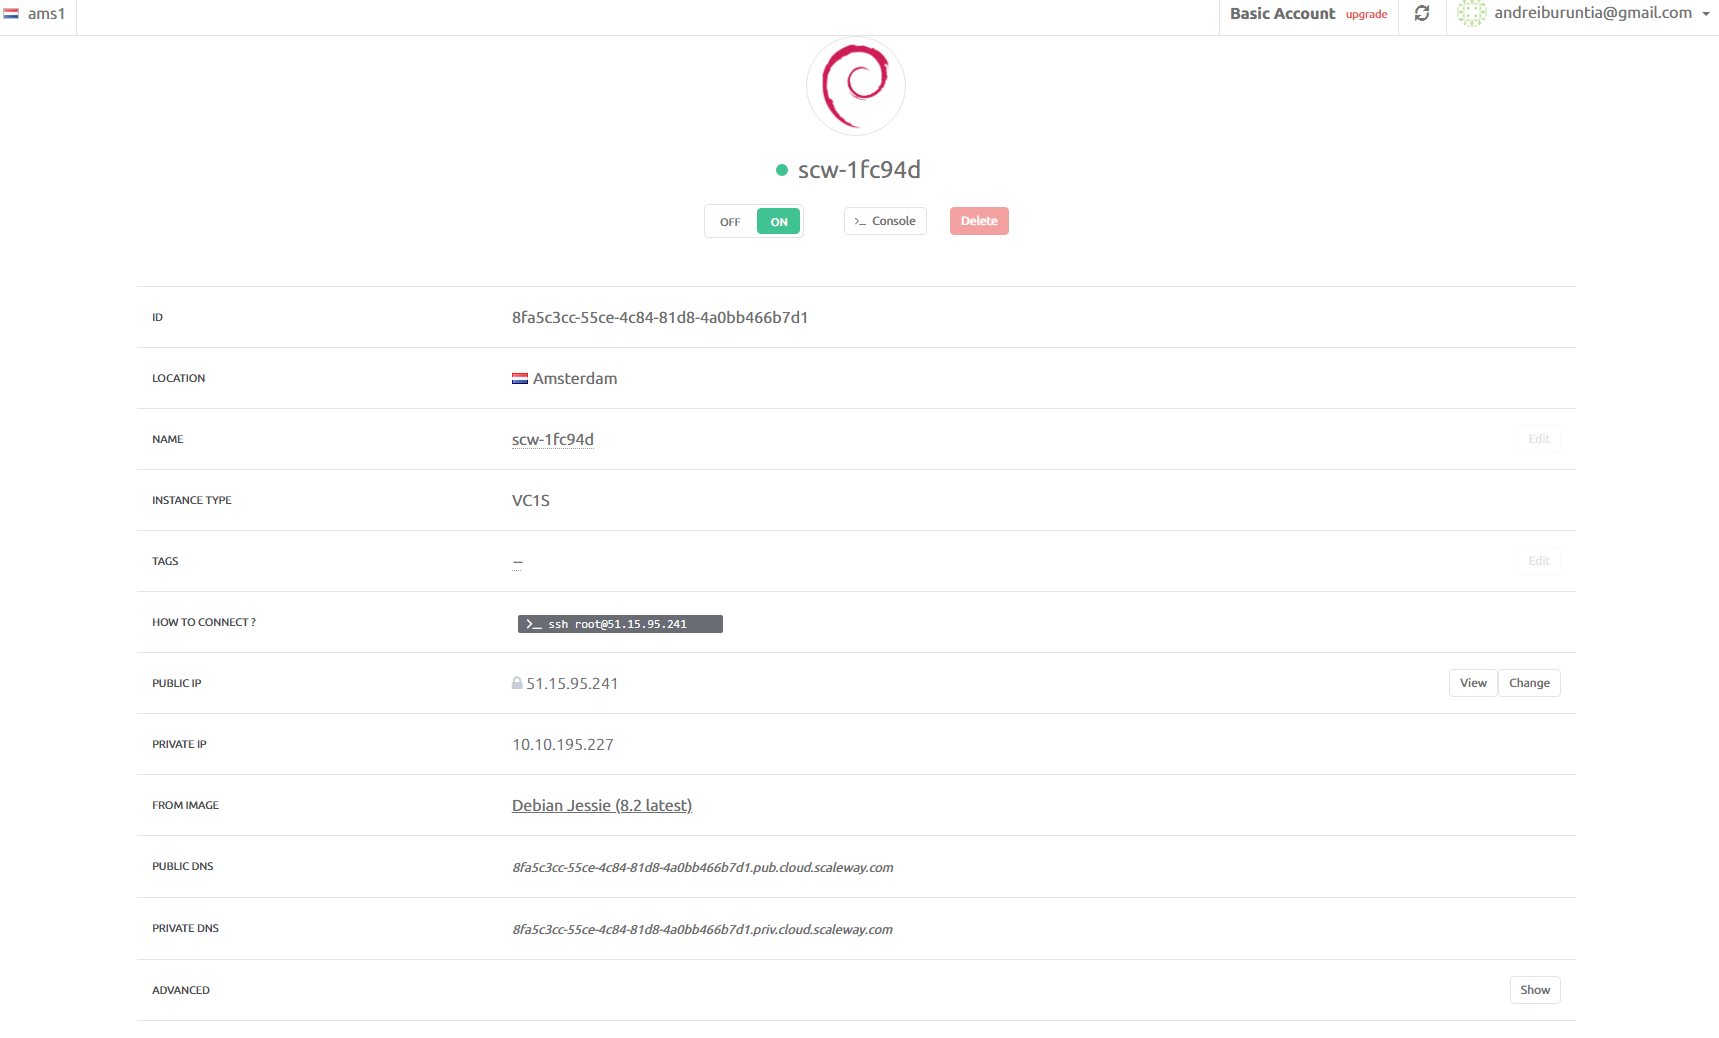
\includegraphics[width=170mm]{scaleway2.png}}
	\caption{Dashboard-ul Scaleway - administrarea unei instanțe de server}
\end{figure}

\chapter{Rezultate}
S-a urmărit și realizat crearea unui sistem de tipărire care trimită date către un agregator spre a fi procesate în scopul ghenerarii de analytics. Prin modificările aduse CUPS, workflow-ul normal nu este modificat în vreun fel, nu apare overhead semnificativ, nu se modifica nici o interfața interna sau externa CUPS și extragerea datelor se face într-o maniera eleganta, non-invaziva. Platforma Kibana și facilitățile ei satisfac cerințele legate de agregarea și vizualizarea datelor colectate din CUPS. Informațiile proprietare Océ nu sunt expuse. Folosirea limbajului Go permite extinderea ulterioara a proiectului cu un cost relativ redus și facilitează posibilitatea folosirii pachetelor și a funcțiilor unui limbaj high-level. Modificările la nivelul clienților sunt aproape inexistente, aceștia trebuind doar sa folosească versiunea modificata de CUPS, care, după cum a fost menționat mai sus, nu alterează comportamentul sau aspectul acestuia. Informațiile colectate sunt suta la suta anonime, nefiind trimise date confidențiale legate de utilizator sau mașina acestuia.

Folosirea ELK stack și CUPS a scăzut considerabil timpul de lucru, scutind dezvoltatorul de implementarea unor astfel de sisteme.

Scalabilitatea proiectul este, în teorie, mărginita doar de capabilitățile de stocare de date și generarea graficelor. O mașina cu un singur nucleu x64, 1 GB de memorie și conexiune de 100Mb/s s-a descurcat în toate testele efectuate. Un eveniment encodat în JSON are dimensiuni de ordinul sutelor de bytes (de obicei mult sub 1kB). Pe 10 GB de stocare persistenta se pot salva peste \begin{math} 10^7 \end{math} astfel de intrări. Având în vedere disponibilitatea spațiului de stocare în zilele noastre, numărul de mai sus respecta orice cerința rezonabila. 

\chapter{Concluzii}
\begin{itemize}
	\item se face evidenta utilitatea folosirii tehnologiilor open-source și clădirea peste sistemelor 'tried and tested'
	\item se remarca avantajele limbajului Go atunci când se dorește folosirea capabilităților unui limbaj de nivel înalt, dar și păstrarea funcționalităților low-level oferite de limbaje precum C
	\item stack-ul ELK este unul robust, solid si eficient
	\item uneltele IPC puse la dispoziție de nucleul Linux (named pipe) sunt suficient de robuste și eficiente pentru a fi folosite cu tehnologii moderne
	\item abundenta dispozitivelor și gradul de dezvoltare rapid a Internetului vor permite colectarea datelor de orice fel
	\item este de menționat cat de importanta a fost abilitatea CUPS de a comunica și rezolva o multitudine de imprimante, fără ca utilizatorul sa facă vreun efort
	\item se remarca versatilitatea și fezabilitatea modelului client-server, folosit aici în doua instante cu constringent-uri și parametrii diferiți
	\item în zilele noastre, un sistem poate colecta, procesa și transmite cu succes date în unități de timp de ordinul sutelor de microsecunde sau zecilor de milisecunde
	\item se remarca flexibilitatea unei licențe permisive precum Apache v2.0
	\item contribuțiile mele strict tehnice la realizarea acestui proiect includ:
		\subitem instalarea si configurarea stack-ului ELK in cloud folosind platforma Scaleway
		\subitem dezvoltarea, configurarea, compilarea si deployment-ul sistemului de operare BuruX bazat pe kernelul Linux
		\subitem modificarea, compilarea si deployment-ul sistemului de printing CUPS
		\subitem conceperea unei arhitecturi/infrastructuri de cominicație
		\subitem dezvoltarea Beater-ului
		\subitem inițializarea si configurarea canalelor de comunicație
		\subitem dezvoltarea de scripturi si programe care să ajute la build sau deployment
		\subitem dezvoltarea de programe care să joace rolul anumitor componente din sistem (stubbing)
		\subitem testarea modulară
		\subitem testarea întregului sistem
		\subitem învățarea tehnologiilor, conceptelor, limbajelor de programare aferente realizării fiecarui din punctele anterior menționate
	\item contribuții de altă natură includ studiul problemei, propunerea si selecția unor soluții fiabile, etc.
\end{itemize}

\chapter{Glosar de termeni}
\begin{itemize}
\item \acrshort{cups} - \acrlong{cups}
\item PDF - Portable Document Format
\item GNU - GNU Not Unix (un acronim recursiv)
\item Linux - familie de sisteme de operare bazate pe nucleul cu același nume
\item OSX - sistem de operare desktop dezvoltat de Apple
\item BSD - Berkeley Software Distribution - sistem de operare Unix-like
\item kernel - nucleul unui sistem de operare
\item Avahi - o implementare de zeroconf networking
\item Golang - limbaj de programare dezvoltat de Google; compilatorul pentru limbajul Go
\item clang - compiler front end pentru backend-ul LLVM
\item Elastic stack - ELK stack - stiva de aplicatii Elastic
\item nginx - web server dezvoltat de Igor Sysoev
\item IPC - inter process communication
\end{itemize}

\listoffigures

\lstlistoflistings

\chapter{Referințe}
\begin{itemize}
\item https://www.scaleway.com/faq/general/
\item Linux Online (2008). "Linux Logos and Mascots". Archived from the original on August 15, 2010. Retrieved August 11, 2009.
\item Torvalds, Linus (January 5, 1992). "Release notes for Linux v0.12". Linux Kernel Archives.
\item "The Linux Kernel Archives: Frequently asked questions". kernel.org. September 2, 2014. Archived from the original on September 5, 2015. Retrieved September 4, 2015.
\item "What Is Linux: An Overview of the Linux Operating System". Linux Foundation. April 3, 2009. Archived from the original on August 13, 2011. Retrieved August 15, 2011.
\item Tung, Liam (July 27, 2017). "Raspberry Pi: 14 million sold, 10 million made in the UK | ZDNet". ZDNet.
\item Upton, Eben (14 March 2018). "Raspberry Pi 3 Model B+ on Sale at USD35". Raspberry Pi Blog. Raspberry Pi .
\item  "Distributed Application Architecture" (PDF). Sun Microsystem. Archived from the original (PDF) on 6 April 2011. Retrieved 2009-06-16.
\item Benatallah, B.; Casati, F.; Toumani, F. (2004). "Web service conversation modeling: A cornerstone for e-business automation". IEEE Internet Computing. 8: 46. doi:10.1109/MIC.2004.1260703.
\end{itemize}
\clearpage

\printglossaries
\end{document}
